\documentclass[submit]{../harvardml}

\course{CS1810-S25}
\assignment{Homework \#2}
\duedate{February 28, 2025 at 11:59 PM}

\usepackage{../common}
\usepackage[OT1]{fontenc}
\usepackage[colorlinks,citecolor=blue,urlcolor=blue]{hyperref}
\usepackage{graphicx}
\usepackage{subfig}
\usepackage{fullpage}
\usepackage{amsmath}
\usepackage{amssymb}
\usepackage{framed}
\usepackage{color}
\usepackage{soul}
\usepackage{todonotes}
\usepackage{listings}
\usepackage{enumitem}
\usepackage{bm}
\usepackage{bbm}
\usepackage{tcolorbox}
\tcbuselibrary{breakable}
\usepackage{float}


\newcommand{\B}{\text{B}}
\newcommand{\Beta}{\text{Beta}}

\usepackage[mmddyyyy,hhmmss]{datetime}

\definecolor{verbgray}{gray}{0.9}

\lstnewenvironment{csv}{%
  \lstset{backgroundcolor=\color{verbgray},
  frame=single,
  framerule=0pt,
  basicstyle=\ttfamily,
  columns=fullflexible}}{}

%%%%%%%%%%%%%%%%%%%%%%%%%%%%%%%%%%%%%%%%%%%
%% Solution environment
\usepackage{xcolor}
\newenvironment{solution}{
    \vspace{2mm}
    \color{blue}\noindent\textbf{Solution}:
}{}
%%%%%%%%%%%%%%%%%%%%%%%%%%%%%%%%%%%%%%%%%%%

\begin{document}

\begin{center}
  {\Large Classification and Bias-Variance Trade-offs}\\
\end{center}

\subsection*{Introduction}

This homework is about classification, bias-variance trade-offs, and
uncertainty quantification.

The datasets that we will be working with relate to astronomical observations and loan applicants.
The first dataset, found at \verb|data/planet-obs.csv|,
contains information on whether a planet was observed (as a binary
variable) at given points in time. This will be used in Problem 1. The
second dataset, available at \verb|data/hr.csv|, details different
loan applicants and their measured debt to income ratio and credit score. You will
work with this data in Problem 3.

As a general note, for classification problems we imagine that we have
the input matrix $\boldX \in \mathbb{R}^{n \times d}$ (or perhaps they
have been mapped to some basis $\bm{\Phi}$, without loss of
generality) with outputs now ``one-hot encoded."  This means that if
there are~$K$ output classes, rather than representing the output
label $y$ as an integer~$\{1,2,\ldots,K\}$, we represent $\boldy$ as a
``one-hot" vector of length~$K$. A ``one-hot" vector is defined as
having every component equal to 0 except for a single component which
has value equal to 1.  For example, if there are $K = 7$ classes and a
particular data point belongs to class 3, then the target vector for
this data point would be~$\boldy = [0,0,1,0,0,0,0]$.  We will define
$C_1$ to be the one-hot vector for the 1st class, $C_2$ for the 2nd
class, etc.  Thus, in the previous example $\boldy = C_3$. If there
are $K$ total classes, then the set of possible labels is $\{C_1
  \ldots C_K \} = \{C_k\}_{k=1}^K$.  Throughout the assignment we will
assume that each label $\boldy \in \{C_k\}_{k=1}^K$ unless otherwise
specified. The most common exception is the case of binary
classification ($K = 2$), in which case labels are the typical
integers $y \in \{0, 1\}$.

\subsection*{Resources and Submission Instructions}

We encourage you to read CS181 Textbook's Chapter 3 for more
information on linear classification, gradient descent, and
classification in the discriminative setting. Read Chapter 2.8 for
more information on the trade-offs between bias and variance.

In problems 1 and 3, you may use \texttt{numpy} or \texttt{scipy}, but
not \texttt{scipy.optimize} or \texttt{sklearn}. Example code is given
in the provided notebook. \textbf{We highly recommend that you use Google Colab for problems 1 and 3 to avoid numerical stability issues.}

Please type your solutions after the corresponding problems using this
\LaTeX\ template, and start each problem on a new page.

Please submit the \textbf{writeup PDF to the Gradescope assignment
  `HW2'}. Remember to assign pages for each question.  Please submit
your \textbf{\LaTeX\ file and code files to the Gradescope assignment
  `HW2 - Supplemental'}. \textbf{You must include your plots in your
  writeup PDF. } The supplemental files will only be checked in
special cases, e.g. honor code issues, etc.

%%%%%%%%%%%%%%%%%%%%%%%%%%%%%%%%%%%%%%%%%%%%%
% Problem 1
%%%%%%%%%%%%%%%%%%%%%%%%%%%%%%%%%%%%%%%%%%%%%

\begin{problem}[Exploring Bias-Variance and Uncertainty]
In this problem, we will explore the bias and variance of a few
different model classes when it comes to logistic regression and
investigate two sources of predictive uncertainty in a synthetic
(made-up) scenario.

We are using a powerful telescope in the northern hemisphere to gather
measurements of some planet of interest. At certain times however, our
telescope is unable to detect the planet due to its positioning around
its star.  The data in \verb|data/planet-obs.csv| records the
observation time in the ``Time" column and whether the planet was
detected in the ``Observed" column (with the value 1 representing that
it was observed).  These observations were taken over a dark, clear
week, which is representative of the region.  Since telescope time is
expensive, we would like to build a model to help us schedule and find
times when we are likely to detect the planet.

\begin{enumerate}
  \item Split the data into 10 mini-datasets of size $N = 30$ (i.e. dataset 1 consists of the first 30 observations, dataset 2 consists of the next 30, etc. This has already been done for you). Consider the three bases $\boldsymbol\phi_1(t) = [1, t]$, $\boldsymbol\phi_2(t) = [1,
          t, t^2]$, and $\boldsymbol\phi_3(t) = [1, t, t^2, t^3, t^4, t^5]$. For each of these bases, fit a logistic regression model using sigmoid($\boldw^\top \boldsymbol\phi(t)$) to each dataset by using gradient descent to
        minimize the negative log-likelihood.  This means you will be
        running gradient descent 10 times for each basis, once for each
        dataset.

        Use the given starting values of $\boldw$ and a learning rate of $\eta=0.001$, take 1,000 update
        steps for each gradient descent run, and make sure to average the
        gradient over the data points at each step. These parameters,
        while not perfect, will ensure your code runs reasonably quickly.

  \item After consulting with a domain expert, we find that the probability of observing the planet is periodic as the planet revolves around its star---we are more likely to observe the planet when it is in front of its star than when it is behind it. In fact, the expert determines that observation follows the generating process $y \sim \text{Bern}(f(t))$, where $f(t) = 0.4 \times \cos(1.1t + 1) + 0.5$ for $t \in [0, 6]$ and $y \in \{0,1\}$. Note that we, the modelers, do not usually see the true data distribution. Knowledge of the true $f(t)$ is only exposed in this problem to allow for verification of the true bias.

        Use the given code to plot the true process versus your learned models. Include your plots in your solution PDF.

        \textbf{In no more than 5 sentences}, explain how bias and variance reflected in the 3 types of curves on the graphs.  How do the fits of the individual and mean prediction functions change?  Keeping in mind that none of the model classes match the true generating process exactly, discuss the extent to which each of the bases approximates the true process.

\end{enumerate}
\end{problem}

\newpage
\begin{framed}
  \noindent\textbf{Problem 1} (cont.)\\
  \begin{enumerate}
    \setcounter{enumi}{2}

    \item If we were to increase the size of each dataset drawn from $N = 30$ to a larger number, how would the bias and variance change for each basis? Why might this be the case? You may experiment with generating your own data that follows the true process and plotting the results, but this is \textbf{not} necessary. \textbf{Your response should not be longer than 5 sentences}.

    \item Consider the test point $t = 0.1$. Using your models trained on basis $\boldsymbol\phi_3$, report the predicted probability of observation of the \textit{first} model (the model trained on the first 30 data points). How can we interpret this probability as a measure of uncertainty? Then, compute the variance of the classification probability over your 10 models at the same point $t = 0.1$. How does this measurement capture another source of uncertainty, and how does this differ from the uncertainty represented by the classification probability? Repeat this process (reporting the first model's classification probability and the variance over the 10 models) for the point $t = 3.2$.

          Compare the uncertainties and their sources at times $t=0.1$ and $t=3.2$.

    \item We now need to make some decisions about when to request time on
          the telescope.  The justifications of your decisions will be sent to
          your funding agency, which will determine whether you will be
          allocated funds to use the telescope for your project. \textbf{In no more than 10 lines}, answer the following questions.
          \begin{itemize}
            \item To identify the ideal time, which model(s) would you use and why?
            \item What time would you request, and why?
            \item Your funding agency suggests using a different telescope in a
                  humid area near the equator. Can you still use your model to
                  determine when the planet is likely to be visible?  Why? Are there
                  adaptations that may be necessary?
            \item You seek out a team that has used the alternative telescope
                  for observing this planet, and they provide you their observation
                  file \verb|data/planet-obs-alternate.csv|.
                  Compare the observations from your telescope to theirs.  What
                  seems to be happening?  What might be an appropriate model for
                  this? Your funding agency asks you to refit your models on these
                  new data.  Do you think this is a reasonable ask, and if so, how
                  will it help you make better decisions about when to request
                  viewing time?  If not, why do you think the additional modeling
                  will not help? You do \emph{not} need to do any modeling for this
                  question!

          \end{itemize}
          In these questions, we are looking for your reasoning; there may be
          more than one valid answer.

  \end{enumerate}
\end{framed}

\newpage

\begin{solution}
\begin{tcolorbox}[colback=white,breakable]

\textbf{Part 1:}  
The logistic regression models were fit on 10 mini-datasets using three bases. This section primarily verifies that the implementation correctly minimizes the negative log-likelihood via gradient descent.

\vspace{2mm}
\textbf{Part 2:}  
\begin{figure}[H]
    \centering
    \subfloat[Basis 1 Models]{%
        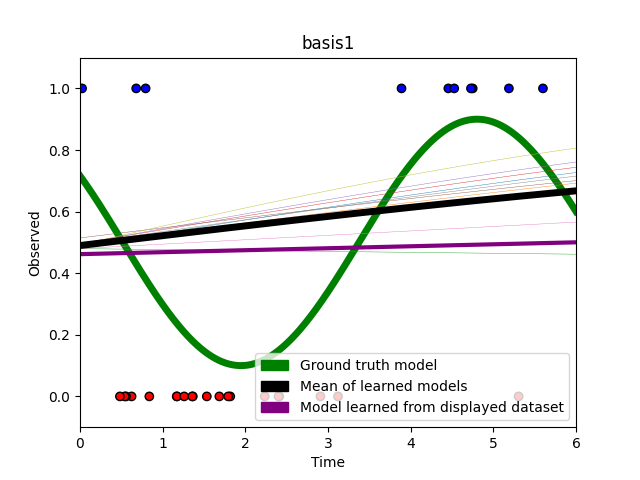
\includegraphics[width=0.3\textwidth]{img_output/basis1.png}
    }
    \subfloat[Basis 2 Models]{%
        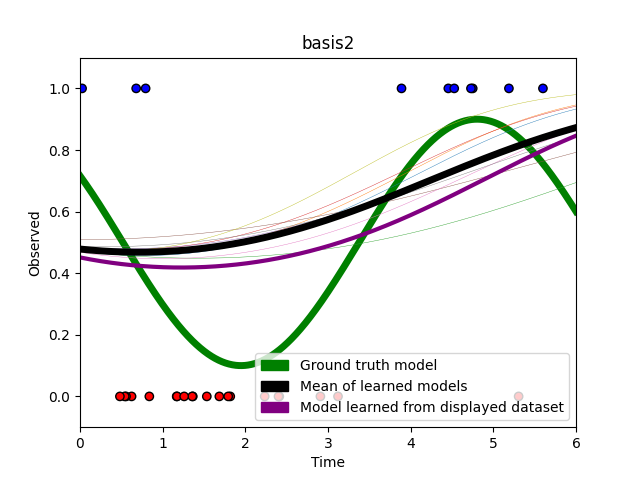
\includegraphics[width=0.3\textwidth]{img_output/basis2.png}
    }
    \subfloat[Basis 3 Models]{%
        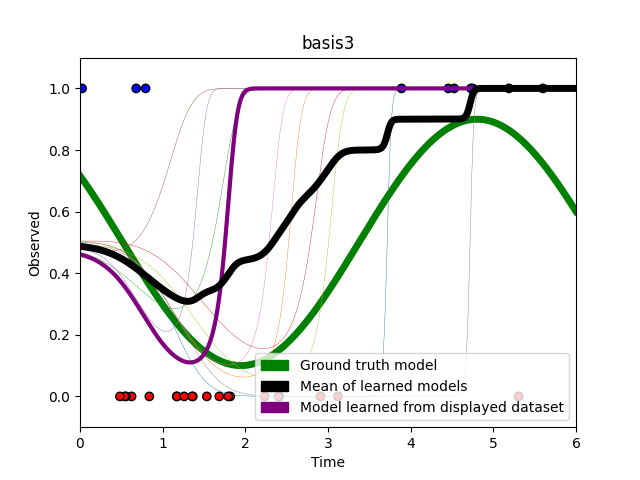
\includegraphics[width=0.3\textwidth]{img_output/basis3.png}
    }
    \caption{Models trained on different polynomial bases showing predictions across 10 different training sets. The green curve is the true generating process $f(t)=0.4\cos(1.1t+1)+0.5$, the purple curve is a representative model from one mini-dataset, and the black curve is the ensemble mean.}
\end{figure}

The curves reveal that the true model (green) has zero bias and variance. The ensemble mean (black) represents an average across datasets, smoothing out idiosyncrasies, while the individual model (purple) reflects the specific dataset’s noise. Basis 1, being linear, cannot capture the underlying periodicity and thus has high bias, whereas Basis 2 improves flexibility; Basis 3, with higher-order terms, best approximates the true process but at the expense of increased variance due to overfitting on small datasets.

\vspace{2mm}
\textbf{Part 3:}  
Increasing the dataset size would reduce variance since the estimates become more stable with more data, though inherent model bias (from an inadequate basis) would remain unchanged. Flexible models like Basis 3 already have low bias and would benefit further from decreased variance. Thus, while all models become more reliable with more data, the trade-off between bias and variance depends on the model’s capacity relative to the true process.

\vspace{2mm}
\textbf{Part 4:}  
At $t = 0.1$, the individual model (purple) predicts a probability of approximately 0.45, indicating uncertainty (close to an even chance) which reflects aleatoric uncertainty. The ensemble mean at $t = 0.1$ is about 0.5 with a noticeable variance across models, capturing epistemic uncertainty due to limited data variability. At $t = 3.2$, the individual model predicts nearly 1, while the ensemble mean is around 0.8, showing increased confidence yet still some dispersion among models. These differences highlight that single-model predictions can be overconfident, whereas ensemble variance reveals uncertainty in regions with less training data.

\vspace{2mm}
\textbf{Part 5 (Decision-Making):}
\begin{itemize}
    \item I would rely on the ensemble prediction of the flexible (Basis 3) model, as it best captures the periodic behavior with lower bias.
    \item I would request telescope time around $t=3.2$, where the ensemble predicts a high probability of observing the planet.
    \item Although the model was trained on our northern telescope data, the underlying periodic process is physical, so with proper recalibration it could be adapted for an equatorial telescope.
    \item Comparing our data with the alternate telescope’s observations reveals systematic differences likely due to atmospheric and instrumental variations; a hierarchical model might better account for these factors.
    \item Re-fitting models on the alternate data would help adjust for these differences, leading to more informed scheduling decisions.
\end{itemize}

\end{tcolorbox}
\end{solution}

%%%%%%%%%%%%%%%%%%%%%%%%%%%%%%%%%%%%%%%%%%%%%
% Problem 2
%%%%%%%%%%%%%%%%%%%%%%%%%%%%%%%%%%%%%%%%%%%%%

\begin{problem}[Maximum likelihood in classification]

Consider now a generative $K$-class model.  We adopt class prior
$p(\boldy = C_k; \bpi) = \pi_k$ for all $k \in \{1, \ldots, K\}$
(where $\pi_k$ is a parameter of the prior).
Let  $p(\boldx|\boldy=C_k)$ denote
the class-conditional density of features $\boldx$ (in this
case for class $C_k$). Consider the data set $D = \{(\boldx_i,
  \boldy_i)\}_{i=1}^n$ where as above $\boldy_i \in \{C_k\}_{k=1}^K$ is
encoded as a one-hot target vector and the data are independent.

\begin{enumerate}
  \item Write out the log-likelihood of the data set, $\ln p(D ; \bpi)$.

  \item Since the prior forms a distribution, it has the constraint that
        $\sum_k\pi_k - 1 = 0$.  Using the hint on
        Lagrange multipliers below, give the
        expression for the maximum-likelihood estimator for the prior
        class-membership probabilities, i.e.
        $\hat \pi_k.$
        Make sure to write out the intermediary equation you need
        to solve to obtain this estimator. Briefly state why your final answer is intuitive.
\end{enumerate}

For the remaining questions, let the
class-conditional probabilities be Gaussian distributions with
the same covariance matrix
$$p(\boldx | \boldy = C_k) = \mathcal{N}(\boldx |  \bmu_k, \bSigma), \text{\ for\ }k \in \{1,\ldots, K\}$$
and different means $\bmu_k$ for each class.

\begin{enumerate}
  \item[3.] Derive the gradient of the log-likelihood with respect to vector $\bmu_k$.
    Write the expression in matrix form as a function of the variables defined
    throughout this exercise. Simplify as much as possible for full credit.
  \item[4.] Derive the maximum-likelihood estimator $\hat{\mu}_k$ for vector $\bmu_k$. Briefly state why your final answer is intuitive.
  \item[5.] Derive the gradient for the log-likelihood with respect to the
    covariance matrix $\bSigma$ (i.e., looking
    to find an MLE for the covariance).
    Since you are differentiating with respect to a
    \emph{matrix}, the resulting expression should be a matrix!
    %
  \item[6.] Derive the maximum likelihood estimator $\hat{\Sigma}$ of the covariance matrix.
\end{enumerate}

\paragraph{Hint: Lagrange Multipliers.} Lagrange Multipliers are a method for
optimizing a function $f$ with respect to an
equality constraint, i.e.
\[\min_{\boldx} f(\boldx)\ \text{s.t.}\ g(\boldx) = 0.\]

This can be turned into an unconstrained problem by introducing a
Lagrange multiplier $\lambda$ and constructing the Lagrangian function,
\[L(\boldx, \lambda) =  f(\boldx) + \lambda g(\boldx).\]

It can be shown that it is a necessary condition that the optimum
is a critical point of this new function. We can find this point by solving two equations:

\[\frac{\partial L(\boldx, \lambda)}{\partial  \boldx} = 0  \ \ \text{and}\  \  \frac{\partial L(\boldx, \lambda)}{\partial \lambda} = 0 \]


\paragraph{Cookbook formulas.} Here are some formulas you might want to consider
using to compute difficult gradients. You can use them  in the homework
without proof. If you are looking to hone your matrix calculus skills, try to
find different ways to prove these formulas yourself (will not be part of the
evaluation of this homework). In general, you can use any formula from the matrix cookbook,
as long as you cite it. We opt for the following common notation:
$\boldX^{-\top} := (\boldX^{\top})^{-1}$
\begin{align*}
   & \frac{\partial \bolda^\top \boldX^{-1} \boldb}{\partial \boldX} = - \boldX^{-\top} \bolda \boldb^\top \boldX^{-\top} \\
   & \frac{\partial \ln | \det (\boldX) |}{\partial \boldX} = \boldX^{-\top}
\end{align*}
\end{problem}

\newpage

\begin{solution}
	

We consider a $K$-class generative model with class prior
\[
p(\vec{y}=C_k;\vec{\pi}) = \pi_k,
\]
and class-conditional density $p(\vec{x}|\vec{y}=C_k)$. The dataset is 
\[
D = \{(\vec{x}_i,\vec{y}_i)\}_{i=1}^n,
\]
with $\vec{y}_i$ one-hot encoded so that
\[
y_{ik} = \begin{cases} 1, & \text{if } \vec{y}_i = C_k, \\ 0, & \text{otherwise.} \end{cases}
\]

The joint probability for a single observation is
\[
p(\vec{x}_i,\vec{y}_i;\vec{\pi}) = \prod_{k=1}^K \left[\pi_k\, p(\vec{x}_i|\vec{y}_i=C_k)\right]^{y_{ik}},
\]
so that the likelihood for the entire dataset is
\[
p(D;\vec{\pi}) = \prod_{i=1}^n \prod_{k=1}^K \left[\pi_k\, p(\vec{x}_i|\vec{y}_i=C_k)\right]^{y_{ik}},
\]
and taking logarithms we obtain
\[
\ln p(D;\vec{\pi}) = \sum_{i=1}^n \sum_{k=1}^K y_{ik}\Bigl(\ln \pi_k + \ln p(\vec{x}_i|\vec{y}_i=C_k)\Bigr).
\]

For the maximum likelihood estimation of $\vec{\pi}$: 
\[
\sum_{k=1}^K \pi_k = 1.
\]
Define
\[
n_k = \sum_{i=1}^n y_{ik}.
\]
we form the Lagrangian
\[
L(\vec{\pi},\lambda) = \sum_{i=1}^n \sum_{k=1}^K y_{ik}\ln \pi_k + \lambda\Bigl(\sum_{k=1}^K \pi_k - 1\Bigr).
\]
Differentiating wrt $\pi_k$ gives
\[
\frac{\partial L}{\partial \pi_k} = \frac{n_k}{\pi_k} + \lambda = 0 \quad \Longrightarrow \quad \pi_k = -\frac{n_k}{\lambda}.
\]
Using the constraint,
\[
\sum_{k=1}^K \pi_k = -\frac{1}{\lambda}\sum_{k=1}^K n_k = -\frac{n}{\lambda} = 1,
\]
so that $\lambda = -n$ and hence
\[
\hat{\pi}_k = \frac{n_k}{n}.
\]
This is intuitive because the prior for class $C_k$ is estimated by the fraction of data points in that class.

Next assume the class-conditional densities are Gaussian,
\[
p(\vec{x}|\vec{y}=C_k)=\mathcal{N}(\vec{x}|\vec{\mu}_k,\vec{\Sigma}),
\]
with
\[
\mathcal{N}(\vec{x}|\vec{\mu}_k,\vec{\Sigma}) = \frac{1}{(2\pi)^{d/2}|\vec{\Sigma}|^{1/2}} \exp\!\Bigl[-\frac{1}{2}(\vec{x}-\vec{\mu}_k)^\top \vec{\Sigma}^{-1}(\vec{x}-\vec{\mu}_k)\Bigr].
\]
Ignoring constants independent of $\vec{\mu}_k$, the log-density is
\[
\ln p(\vec{x}_i|\vec{y}_i=C_k) = -\frac{1}{2}(\vec{x}_i-\vec{\mu}_k)^\top \vec{\Sigma}^{-1}(\vec{x}_i-\vec{\mu}_k).
\]
Thus, the contribution to the log-likelihood from class $C_k$ is
\[
\ell_k(\vec{\mu}_k) = \sum_{i=1}^n y_{ik}\Bigl[-\frac{1}{2}(\vec{x}_i-\vec{\mu}_k)^\top \vec{\Sigma}^{-1}(\vec{x}_i-\vec{\mu}_k)\Bigr].
\]
Differentiating with respect to $\vec{\mu}_k$, for a single term we have
\[
\nabla_{\vec{\mu}_k}\Bigl[-\frac{1}{2}(\vec{x}_i-\vec{\mu}_k)^\top \vec{\Sigma}^{-1}(\vec{x}_i-\vec{\mu}_k)\Bigr] = \vec{\Sigma}^{-1}(\vec{x}_i-\vec{\mu}_k).
\]
Summing over all $i$ gives
\[
\nabla_{\vec{\mu}_k}\ln p(D) = \vec{\Sigma}^{-1}\Bigl(\sum_{i=1}^n y_{ik}\vec{x}_i - n_k\,\vec{\mu}_k\Bigr).
\]
Setting this equal to zero, we obtain
\[
\sum_{i=1}^n y_{ik}\vec{x}_i = n_k\,\vec{\mu}_k, \quad \hat{\vec{\mu}}_k = \frac{1}{n_k}\sum_{i=1}^n y_{ik}\vec{x}_i.
\]
This is the sample mean of the observations in class $C_k$.

For the covariance matrix, the $\vec{\Sigma}$-dependent part of the log-density is
\[
-\frac{1}{2}\ln\det(2\pi\,\vec{\Sigma}) - \frac{1}{2}(\vec{x}_i-\vec{\mu}_k)^\top \vec{\Sigma}^{-1}(\vec{x}_i-\vec{\mu}_k).
\]
Ignoring constants, the relevant log-likelihood is
\[
L(\vec{\Sigma}) = -\frac{1}{2}\sum_{i=1}^n \sum_{k=1}^K y_{ik}\Bigl[\ln\det(\vec{\Sigma}) + (\vec{x}_i-\vec{\mu}_k)^\top \vec{\Sigma}^{-1}(\vec{x}_i-\vec{\mu}_k)\Bigr].
\]
The derivative of $\ln\det(\vec{\Sigma})$ with respect to $\vec{\Sigma}$ is $\vec{\Sigma}^{-1}$, and the derivative of the quadratic term is
\[
\frac{1}{2}\vec{\Sigma}^{-1}(\vec{x}_i-\vec{\mu}_k)(\vec{x}_i-\vec{\mu}_k)^\top\vec{\Sigma}^{-1}.
\]
Summing over all data points, the gradient is
\[
\nabla_{\vec{\Sigma}}\ln p(D) = -\frac{n}{2}\,\vec{\Sigma}^{-1} + \frac{1}{2}\,\vec{\Sigma}^{-1}\Biggl[\sum_{i=1}^n \sum_{k=1}^K y_{ik}(\vec{x}_i-\vec{\mu}_k)(\vec{x}_i-\vec{\mu}_k)^\top\Biggr]\vec{\Sigma}^{-1}.
\]
Setting this equal to zero yields
\[
\vec{\Sigma}^{-1}\Biggl[\sum_{i=1}^n \sum_{k=1}^K y_{ik}(\vec{x}_i-\vec{\mu}_k)(\vec{x}_i-\vec{\mu}_k)^\top\Biggr] = n\,\mathbf{I}.
\]
Multiplying by $\vec{\Sigma}$ gives
\[
\sum_{i=1}^n \sum_{k=1}^K y_{ik}(\vec{x}_i-\vec{\mu}_k)(\vec{x}_i-\vec{\mu}_k)^\top = n\,\vec{\Sigma},
\]
so that the maximum likelihood estimator for $\vec{\Sigma}$ is
\[
\hat{\vec{\Sigma}} = \frac{1}{n}\sum_{i=1}^n \sum_{k=1}^K y_{ik}(\vec{x}_i-\vec{\mu}_k)(\vec{x}_i-\vec{\mu}_k)^\top.
\]
This  estimator combines the information from all classes.

\end{solution}

%%%%%%%%%%%%%%%%%%%%%%%%%%%%%%%%%%%%%%%%%%%%%
% Problem 3
%%%%%%%%%%%%%%%%%%%%%%%%%%%%%%%%%%%%%%%%%%%%%

\begin{problem}[Classifying Loan Applicants]
In this problem, you will code up three different classifiers to classify different types of loan applicants. The file \verb|data/hr.csv| contains data on debt to income ratio measured in tenths of a percent and credit score. The data can be plotted on these two axes:
\begin{center}
  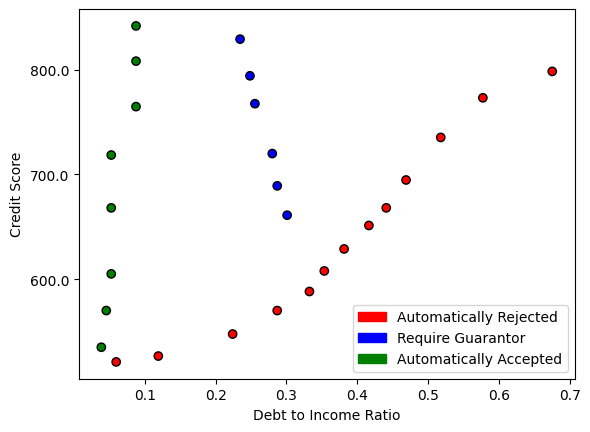
\includegraphics[width=.5\textwidth]{img_input/credit.png}
\end{center}

Please implement the following classifiers in the \verb|SoftmaxRegression| and \verb|KNNClassifier| classes.

\textbf{For this problem, apply the following transformation to all data:}

$$\phi(\boldx) = \left[x_1 \cdot \frac{200}{7}-7.5, \frac{x_2-500}{140}+0.5\right]^\top$$

  where $x_1$ and $x_2$ represent the values for debt to income ratio and credit score, respectively.
  
  This transformation has been applied to the data for you in the notebook.

\begin{enumerate}[label=\alph*)]

  \item \textbf{A generative classifier with Gaussian class-conditional
          densities with a \textit{shared covariance} matrix} across all classes.
        Feel free to re-use your Problem 2 results.

  \item \textbf{Another generative classifier with Gaussian class-conditional densities , but now
          with a \textit{separate covariance} matrix} learned for each class. (Note:
        The staff implementation can switch between the two Gaussian generative classifiers with just a
        few lines of code.)

  \item \textbf{A multi-class logistic regression classifier} using the softmax activation function. In your implementation of gradient descent, \textbf{make sure to include a bias term and use L2 regularization} with regularization parameter $\lambda = 0.001$. Limit the number of iterations of gradient descent to 200,000, and set the learning rate to be $\eta = 0.001$.

  \item \textbf{Another multi-class logistic regression classifier} with the additional feature map:
  $$\phi(\boldx) = [\ln (x_1+10), x_2^2]^\top$$
  where $x_1$ and $x_2$ represent the values for debt to income ratio and credit score, respectively.

  \item \textbf{A kNN classifier} in which you classify based on the $k = 1$ and $k = 5$ nearest neighbors and the following distance function: $$dist(loan\_app_1, loan\_app_2) = \frac{(debt_1 - debt_2)^2}{9} + (credit_1 - credit_2)^2$$
        where nearest neighbors are those with the smallest distances from a given point.

        Note 1: When there are more than two labels, no label may have the
        majority of neighbors.  Use the label that has the most votes among
        the neighbors as the choice of label.

        Note 2: The grid of points for which you are making predictions
        should be interpreted as our test space.  Thus, it is not necessary
        to make a test point that happens to be on top of a training point
        (i.e. ignore itself when selecting neighbors).
\end{enumerate}
\end{problem}

\newpage

\begin{framed}
  \noindent\textbf{Problem 3} (cont.)\\

After implementing the above classifiers, complete the following exercises:
  \begin{enumerate}

      \item Plot the decision boundaries generated by each classifier for the dataset. Include them in your PDF.
            Identify the similarities and differences among the classifiers. What explains the differences---in particular, which aspects or properties of each model dictate the shape of its decision boundary?
    
      \item
    
            Consider a loan applicant with Debt to Income Ratio 0.32 and Credit Score 350. To which class does each classifier assign this applicant? Report the classification probabilities of this applicant for models (c) and (d).
            
            Interpret how each model makes its classification decision. What else should we, the modelers, be aware of when making predictions on a point "far" from our training data? \textbf{Your response should not be longer than 5 sentences.}

    \item
        Can you think of any ethical problem that might arise from using this classifier to make loan decisions? You may approach this from any angle you like. For instance, can you think of someone who might have a low credit score and high debt-to-income ratio that you believe should nonetheless be offered a loan? Are there other variables that should be accounted for to ensure fair decisions? Are credit scores and debt-to-income ratio good bases for loan decisions? More generally, is using a classifier trained on past decisions to determine loan eligibility problematic in any way?
    \end{enumerate}
\end{framed}

\newpage

\begin{solution}
  \begin{tcolorbox}[colback=white,breakable]
  
  \textbf{(a) Decision Boundary Analysis:} \\
  The decision boundaries produced by each classifier reveal their distinctive characteristics. Gaussian generative models create smooth, elliptical boundaries, with the shared covariance model enforcing similar boundary shapes across all classes, while the separate covariance model allows each class to develop uniquely oriented decision regions. The multi-class logistic regression classifiers generate linear boundaries in the transformed feature space, though the additional feature mapping introduces subtle nonlinearities. In stark contrast, the kNN classifiers produce highly irregular, locally adaptive boundaries that closely follow the training data distribution. These fundamental differences stem from each model's underlying mathematical formulation—parametric models impose specific functional forms while non-parametric approaches like kNN allow the data to directly shape the decision surface.
  
  \begin{figure}[H]
      \centering
      \begin{minipage}[b]{0.48\textwidth}
          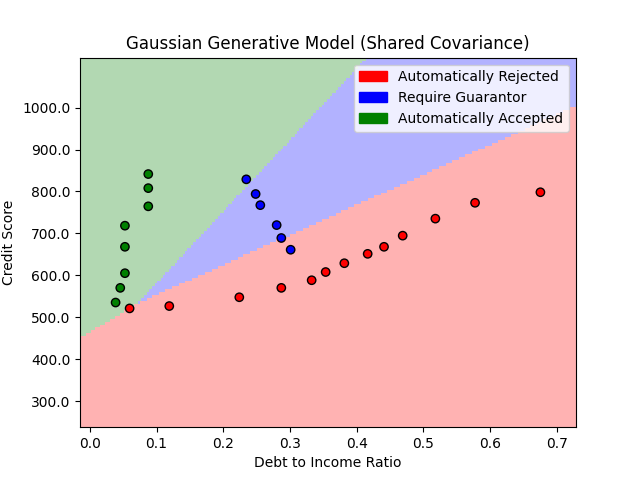
\includegraphics[width=\textwidth]{img_output/Gaussian Generative Model (Shared Covariance).png}
          \caption{Gaussian Generative Model (Shared Covariance)}
      \end{minipage}
      \hfill
      \begin{minipage}[b]{0.48\textwidth}
          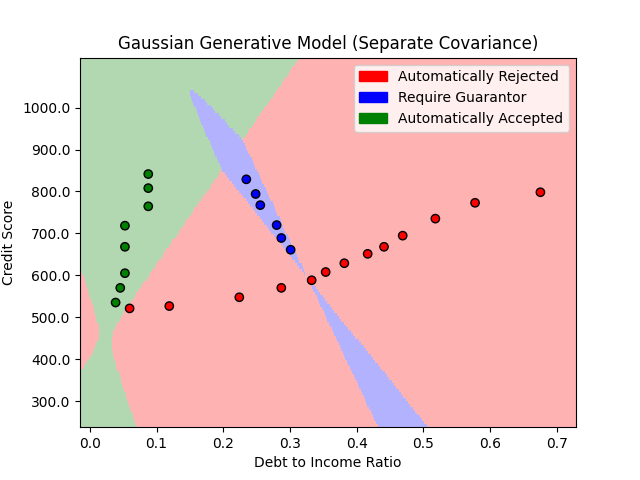
\includegraphics[width=\textwidth]{img_output/Gaussian Generative Model (Separate Covariance).png}
          \caption{Gaussian Generative Model (Separate Covariance)}
      \end{minipage}
  \end{figure}
  
  \begin{figure}[H]
      \centering
      \begin{minipage}[b]{0.48\textwidth}
          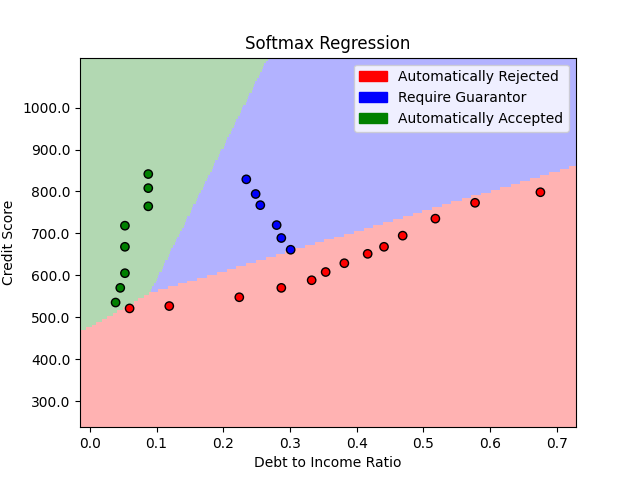
\includegraphics[width=\textwidth]{img_output/Softmax Regression.png}
          \caption{Softmax Regression}
      \end{minipage}
      \hfill
      \begin{minipage}[b]{0.48\textwidth}
          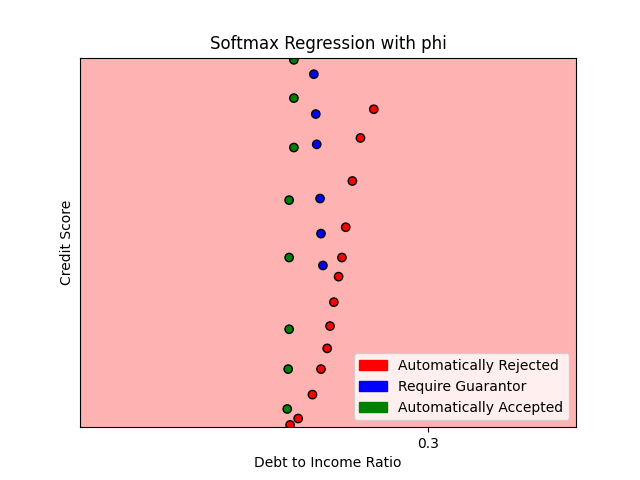
\includegraphics[width=\textwidth]{img_output/Softmax Regression with phi.png}
          \caption{Softmax Regression with Additional Feature Mapping}
      \end{minipage}
  \end{figure}
  
  \begin{figure}[H]
      \centering
      \begin{minipage}[b]{0.48\textwidth}
          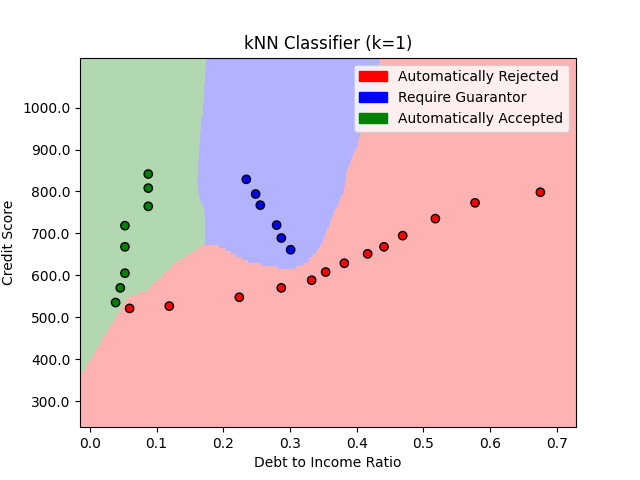
\includegraphics[width=\textwidth]{img_output/kNN Classifier (k=1).png}
          \caption{kNN Classifier (k=1)}
      \end{minipage}
      \hfill
      \begin{minipage}[b]{0.48\textwidth}
          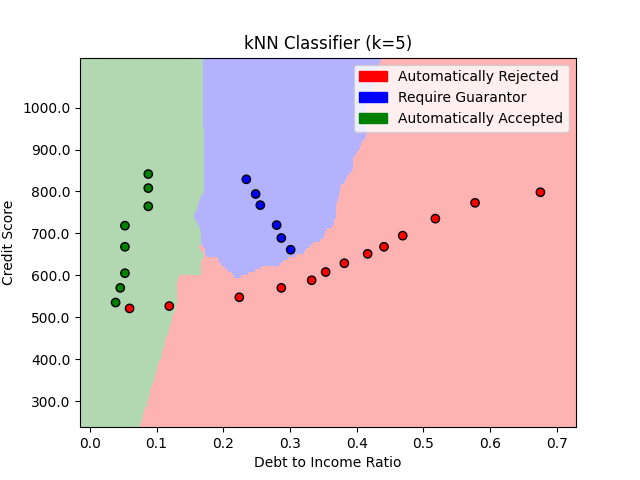
\includegraphics[width=\textwidth]{img_output/kNN Classifier (k=5).png}
          \caption{kNN Classifier (k=5)}
      \end{minipage}
  \end{figure}
  
  \vspace{2mm}
  \textbf{(b) Prediction for a New Applicant:} \\
  When evaluating a loan applicant with a Debt to Income Ratio of 0.32 and Credit Score of 350, all implemented classifiers unanimously assign the applicant to class 0 (Automatically Rejected). The softmax regression models assign a probability virtually equal to 1 for class 0, indicating exceptional confidence in this prediction. This unanimous rejection occurs because the applicant's features place them in a sparse region of the feature space, far from the training examples. This case highlights the critical issue of extrapolation reliability—models can produce deceptively confident predictions in regions with limited training data, underscoring the importance of uncertainty quantification when deploying such models in high-stakes financial contexts.
  
  \vspace{2mm}
  \textbf{(c) Ethical Considerations:} \\
  Basing loan decisions exclusively on debt-to-income ratio and credit score raises significant ethical concerns, as these metrics alone cannot capture the nuanced financial circumstances of applicants. This approach may systematically disadvantage individuals from historically marginalized communities, those with limited credit histories, or people experiencing temporary financial hardships despite strong repayment potential. Furthermore, training classifiers on historical lending decisions risks perpetuating and amplifying existing discriminatory patterns. A more equitable approach would incorporate alternative financial indicators, contextual factors like employment stability and future earning potential, and regular algorithmic fairness audits to ensure the model doesn't disproportionately impact protected groups.
  
  \end{tcolorbox}
  \end{solution}

\newpage
%%%%%%%%%%%%%%%%%%%%%%%%%%%%%%%%%%%%%%%%%%%%%
% Name and Calibration
%%%%%%%%%%%%%%%%%%%%%%%%%%%%%%%%%%%%%%%%%%%%%
\newpage

\textbf{Name}: matt krasnow

\textbf{Collaborators and Resources}: Textbook, online lectures. Used ChatGPT to scan my handwritten work into LaTeX. Stack Overflow for help with LaTeX.

\end{document}
